%% Draft for Electric Power Systems Research (Elsevier). Every number comes from generated/results_macros.tex (tools/build_paper_macros_v5.py).
%% Citations marked \tc{...} are placeholders: the reference list is not yet verified (see REFERENCES_TO_VERIFY.md).
\documentclass[preprint,12pt,authoryear]{elsarticle}
\usepackage{amsmath,amssymb,booktabs,float,graphicx,xcolor,tikz,array,url}
\usetikzlibrary{arrows.meta,positioning,calc}
% generated by tools/build_paper_macros_v5.py - do not edit
\newcommand{\catExtInrush}{88.3}
\newcommand{\catHiz}{65.8}
\newcommand{\catLvSolid}{94.7}
\newcommand{\catNcat}{16}
\newcommand{\catSotf}{90.0}
\newcommand{\clAgree}{50}
\newcommand{\clBPass}{12}
\newcommand{\clBTotal}{12}
\newcommand{\clDtMax}{0.30}
\newcommand{\clDtMed}{0.00}
\newcommand{\clMirOk}{49}
\newcommand{\clNfail}{2}
\newcommand{\clSimOk}{49}
\newcommand{\clTotal}{50}
\newcommand{\cpADep}{94.56}
\newcommand{\cpASec}{98.79}
\newcommand{\cpBDep}{95.33}
\newcommand{\cpBSec}{96.73}
\newcommand{\cpDep}{94.78}
\newcommand{\cpSec}{98.22}
\newcommand{\cvGateDep}{88.38}
\newcommand{\cvGateFalse}{34}
\newcommand{\cvGateMed}{16.2}
\newcommand{\cvGateMissed}{436}
\newcommand{\cvGateSec}{99.43}
\newcommand{\cvHarmDep}{85.93}
\newcommand{\cvHarmSec}{99.40}
\newcommand{\cvHybDep}{92.99}
\newcommand{\cvHybDepSD}{3.60}
\newcommand{\cvHybFalse}{62}
\newcommand{\cvHybMed}{16.2}
\newcommand{\cvHybMissed}{263}
\newcommand{\cvHybSec}{98.96}
\newcommand{\cvHybSecSD}{0.81}
\newcommand{\cvLstmDep}{97.68}
\newcommand{\cvLstmFalse}{262}
\newcommand{\cvLstmMed}{15.6}
\newcommand{\cvLstmMissed}{83}
\newcommand{\cvLstmSec}{95.60}
\newcommand{\cvNeval}{3238}
\newcommand{\cvNfault}{1251}
\newcommand{\cvNfold}{15}
\newcommand{\cvNhealthy}{1987}
\newcommand{\cvNseed}{3}
\newcommand{\cvTaDep}{80.34}
\newcommand{\cvTaFalse}{2181}
\newcommand{\cvTaMed}{1.2}
\newcommand{\cvTaMissed}{405}
\newcommand{\cvTaSec}{63.41}
\newcommand{\dsMainA}{3340}
\newcommand{\dsMainB}{1290}
\newcommand{\dwellN}{20}
\newcommand{\eOneDep}{91.98}
\newcommand{\eOneDepLoss}{47}
\newcommand{\eOneDepP}{7.6e-07}
\newcommand{\eOneDepWins}{9}
\newcommand{\eOneOodSec}{92.7}
\newcommand{\eOneSec}{99.38}
\newcommand{\latCMax}{376.9}
\newcommand{\latCMed}{175.9}
\newcommand{\latCPnn}{228.9}
\newcommand{\latOnnxMed}{139.6}
\newcommand{\latOnnxPnn}{218.9}
\newcommand{\latPeriod}{625}
\newcommand{\looABDep}{93.10}
\newcommand{\looABSec}{89.79}
\newcommand{\looBADep}{62.51}
\newcommand{\looBASec}{97.28}
\newcommand{\mcPDepBase}{85.93}
\newcommand{\mcPDepLoss}{1}
\newcommand{\mcPDepN}{1251}
\newcommand{\mcPDepP}{4.1e-29}
\newcommand{\mcPDepProp}{93.92}
\newcommand{\mcPDepWins}{101}
\newcommand{\mcPSecBase}{99.40}
\newcommand{\mcPSecLoss}{17}
\newcommand{\mcPSecN}{1987}
\newcommand{\mcPSecP}{0.46}
\newcommand{\mcPSecProp}{99.14}
\newcommand{\mcPSecWins}{12}
\newcommand{\mcUDepBase}{80.34}
\newcommand{\mcUDepLoss}{9}
\newcommand{\mcUDepN}{1251}
\newcommand{\mcUDepP}{3.6e-42}
\newcommand{\mcUDepProp}{93.92}
\newcommand{\mcUDepWins}{179}
\newcommand{\mcUSecBase}{63.41}
\newcommand{\mcUSecLoss}{8}
\newcommand{\mcUSecN}{1987}
\newcommand{\mcUSecP}{1.1e-200}
\newcommand{\mcUSecProp}{99.14}
\newcommand{\mcUSecWins}{718}
\newcommand{\netMacs}{1.67}
\newcommand{\netParams}{58241}
\newcommand{\oodBlockADep}{100.0}
\newcommand{\oodBlockASec}{96.7}
\newcommand{\oodBlockBDep}{100.0}
\newcommand{\oodBlockBSec}{100.0}
\newcommand{\oodBlockCDep}{100.0}
\newcommand{\oodBlockCSec}{96.7}
\newcommand{\oodBlockDDep}{96.7}
\newcommand{\oodBlockDSec}{93.3}
\newcommand{\oodBlockEDep}{93.1}
\newcommand{\oodBlockESec}{93.3}
\newcommand{\oodDep}{98.0}
\newcommand{\oodFalse}{6}
\newcommand{\oodMed}{17.5}
\newcommand{\oodMissed}{3}
\newcommand{\oodN}{299}
\newcommand{\oodSec}{96.0}
\newcommand{\tfA}{7.39}
\newcommand{\tfB}{8.64}
\newcommand{\thrAi}{0.9950}
\newcommand{\thrSolo}{0.9980}
\newcommand{\tpFalseAll}{89}
\newcommand{\tpFalseExt}{89}
\newcommand{\tpFalseSolo}{87}
\newcommand{\tpHighsetDep}{50.3}
\newcommand{\tpNoSoloDep}{90.47}
\newcommand{\tpNoSoloSec}{99.21}
\newcommand{\tpSoloOnlyFaults}{11}
\newcommand{\zsHarmDep}{94.12}
\newcommand{\zsHarmFalse}{8}
\newcommand{\zsHarmMissed}{29}
\newcommand{\zsHarmSec}{98.95}
\newcommand{\zsLstmDep}{92.90}
\newcommand{\zsLstmFalse}{97}
\newcommand{\zsLstmMissed}{35}
\newcommand{\zsLstmSec}{87.30}
\newcommand{\zsNfault}{493}
\newcommand{\zsNhealthy}{764}
\newcommand{\zsPropDep}{92.70}
\newcommand{\zsPropFalse}{89}
\newcommand{\zsPropMissed}{36}
\newcommand{\zsPropSec}{88.35}
\newcommand{\zsTaDep}{89.45}
\newcommand{\zsTaFalse}{290}
\newcommand{\zsTaMissed}{29}
\newcommand{\zsTaSec}{62.04}

\newcommand{\tc}[1]{\textcolor{red}{[cite: #1]}}
\journal{Electric Power Systems Research}

\begin{document}
\begin{frontmatter}
\title{Dual-path supervision of a transformer differential relay by a wavelet-feature LSTM: a leak-free evaluation on two simulated plants}
\author[inst1]{Author One}
\author[inst1]{Author Two}
\affiliation[inst1]{organization={Department, University}, city={City}, country={Country}}
\begin{abstract}
A conventional transformer differential relay (87T) with percentage restraint operates on inrush, over-excitation and current-transformer (CT) saturation unless harmonic restraint is added; learned classifiers can discriminate these conditions but are commonly evaluated on random splits of correlated windows against weak baselines. This paper describes a supervisory relay in which a long short-term memory (LSTM) network on wavelet and second-harmonic features confirms the 87T vote and, separately, trips on its own when a persistence-filtered score exceeds a higher threshold, while the high-set element stays outside the network. The relay is evaluated on two Simulink/SimPowerSystems transformers (300\,MVA YNd1 and 40\,MVA Dyn11) with CTs sized to be linear for the through-fault current at nominal burden, using trace-grouped cross-validation, onset-based labels, thresholds tuned on validation traces only, an out-of-distribution set scored once, and a per-phase harmonic-restrained 87T and five literature classifiers as baselines on identical folds. On plant~A (\cvNfold{} fold-models) the relay reaches \cvHybDep\,\% dependability and \cvHybSec\,\% security; the per-phase harmonic 87T reaches \cvHarmDep\,\% and \cvHarmSec\,\%. The dependability difference is significant (paired McNemar, $p=\mcPDepP$), the security difference is not ($p=\mcPSecP$). A model trained on plant~A does not transfer to plant~B (security \zsPropSec\,\%); training on both plants gives \cpDep\,\% and \cpSec\,\%. Limitations: simulation only, two plants, terminal faults, internal high-impedance faults detected in \catHiz\,\% of traces.
\end{abstract}
\begin{keyword}
transformer differential protection \sep inrush \sep CT saturation \sep LSTM \sep wavelet transform \sep evaluation protocol
\end{keyword}
\end{frontmatter}

\section{Introduction}
Differential protection (ANSI 87T) is the main protection of power transformers. Its percentage-restrained characteristic is blocked or restrained against magnetising inrush, over-excitation and CT saturation by harmonic content of the differential current, and these measures trade security against operating speed and sensitivity to internal faults with low current \citep{sharp1958,ieee_c37_91}. A large body of work replaces or supplements the harmonic criteria with wavelet features and classifiers: support vector machines, shallow networks, random forests, convolutional and recurrent networks \tc{transformer differential protection with ML: SVM, ANN, RF, CNN, GRU, LSTM}.

Three problems limit what such studies show. First, the evaluation unit is often a window cut from a small number of simulated cases, so that windows from one case appear in both training and test sets. Second, the baseline is an unrestrained percentage-differential characteristic, not a harmonic-restrained one. Third, the simulated plant is rarely documented to the extent that its through-fault current, CT burden and saturation behaviour can be judged. This paper addresses these points with a stated protocol and a plant that was checked against explicit physics criteria; the DWT\,+\,LSTM feature pipeline itself is not claimed as new.

The contributions are:
\begin{enumerate}
\item a \emph{dual-path supervisory relay}: an 87T-gated AI confirmation, a persistence-filtered AI-alone path for faults below the 87T pickup, and a high-set element that does not depend on the network (Section~\ref{sec:method});
\item a \emph{leak-free evaluation protocol} (Section~\ref{sec:protocol}): trace-grouped cross-validation over three seeds, onset-based labels, thresholds tuned on validation traces only, an out-of-distribution (OOD) set scored once, and undetectable faults reported separately;
\item \emph{baselines on identical folds} with paired statistics: the unrestrained 87T, a per-phase harmonic-restrained 87T and five literature classifiers (Section~\ref{sec:results});
\item a test on a \emph{second transformer}: zero-shot transfer, pooled training and leave-one-plant-out, and a Simulink closed loop that reproduces the offline decisions.
\end{enumerate}
The results do not show that the relay is better than a harmonic-restrained 87T in every respect; Section~\ref{sec:results} states where it is and where it is not.

\section{Related work}
\label{sec:related}
\tc{Harmonic restraint and blocking: second/fifth harmonic, waveform-based, voltage-restrained, flux-based methods}. \tc{Wavelet-based discrimination of inrush and internal faults}. \tc{CT-saturation detection and compensation}. \tc{Machine-learning transformer protection: SVM, ANN, RF, CNN, GRU, LSTM, with the evaluation methods they report}. Leakage between training and test data is a documented source of overstated results in machine-learning studies \citep{kapoor2023}. Block-decomposition and Clarke-wavelet methods are discussed as alternatives in Section~\ref{sec:limits}.

\section{Plants and data}
\label{sec:data}
\subsection{Plants}
Plant~A is a 300\,MVA, 230/11\,kV YNd1 transformer with 5\,A CT secondaries (1\,$\Omega$ nominal burden); plant~B is a 40\,MVA, 132/33\,kV Dyn11 transformer with 1\,A secondaries (2.5\,$\Omega$). Both are SimPowerSystems models with a saturable transformer, six saturable CT subsystems, a series source impedance, a load, breaker-controlled energisation and fault blocks on the LV and HV sides. Transformer reactance is 11\,\% (A) and 10\,\% (B) with $X/R\approx 20$; the earlier version of the plants (2\,\% and 1\,\% leakage) produced through-fault currents of 23.9 and 37.6\,pu and CTs that saturated on every solid external fault, and was discarded.

The CTs are sized so that they are linear in steady state at nominal burden for the maximum symmetrical through-fault, and saturate only with DC offset or increased burden. The following checks were run on each plant before any data was generated: true line currents from V--I blocks (not CT secondaries) give a steady through-fault of \tfA\,pu RMS on plant~A and \tfB\,pu on plant~B; the CT secondary follows the scaled primary within a few per cent at nominal burden; the normal-operation differential residual is below 0.01\,pu; CT ratio drift at 150\,\% load and three times the burden is about 2\,\%. Plant~B does not meet two of the six criteria set in advance (a DC offset at maximum asymmetry does not saturate its CTs at nominal burden, and the ratio drift of 2.02\,\% exceeds the 2\,\% limit by 0.02 points); these are reported as measured (file \texttt{plant\_v5\_checks\_B.txt} in the repository).

\subsection{Scenarios and coverage}
Each trace is 1.1\,s sampled at 1600\,Hz. \catNcat{} scenario categories cover normal operation at 1--130\,\% load, energisation inrush (no-load, loaded, sympathetic recovery after an external fault), over-excitation, external faults (solid, high-impedance, with CT saturation, during inrush), internal faults on the LV and HV side (solid, high-impedance, evolving, switch-on-to-fault, with CT saturation, during inrush). Per trace, load, power factor, noise, CT gain mismatch, CT burden, source strength, frequency, inception angle, residual flux and fault resistance are drawn from stated ranges; high-impedance fault resistance is drawn from bins derived from a sensitivity sweep of the differential current (87T-visible, AI-only, undetectable). Plant~A has \dsMainA{} and plant~B \dsMainB{} traces in the main sets (including top-ups to meet the coverage criteria) plus OOD sets generated with ranges outside the training distribution (extreme load, weak source and frequency offset, extreme CT burden, severe over-excitation, high noise and CT mismatch). A coverage report with eight acceptance criteria (cell counts per scenario group and load bin, inrush angle and flux cells, high-impedance bins, CT-saturation fraction, over-excitation harmonics, realised load, generator checks, true through-fault range) is part of the repository; both plants pass it.

\section{Method}
\label{sec:method}
\subsection{Features}
The plant-compensated differential current (YNd1: matrix on the HV side; Dyn11: matrix on the LV side) is divided by the rated CT secondary current. For each phase a 32-sample window (20\,ms) is decomposed with a two-level Daubechies-4 wavelet; the energies of D1, D2 and A2 enter as $\ln(1+E)$. The ratio of the 100\,Hz to the 50\,Hz DFT magnitude of the window, limited to 2, is added per phase. The feature vector has 12 elements \citep{mallat1989}. The same code path is used by the offline pipeline and the Simulink relay; their features agree with zero error in a parity check on both plants.

\subsection{Network}
A two-layer unidirectional LSTM \citep{hochreiter1997} (hidden size 64) is followed by layer normalisation, a single-head additive attention over the 32 time steps and a two-layer classifier with a sigmoid output; the input is 32 steps of the 12 features. The network has \netParams{} parameters and about \netMacs\,M multiply--accumulate operations per inference.

\subsection{Decision logic}
\begin{figure}[t]\centering
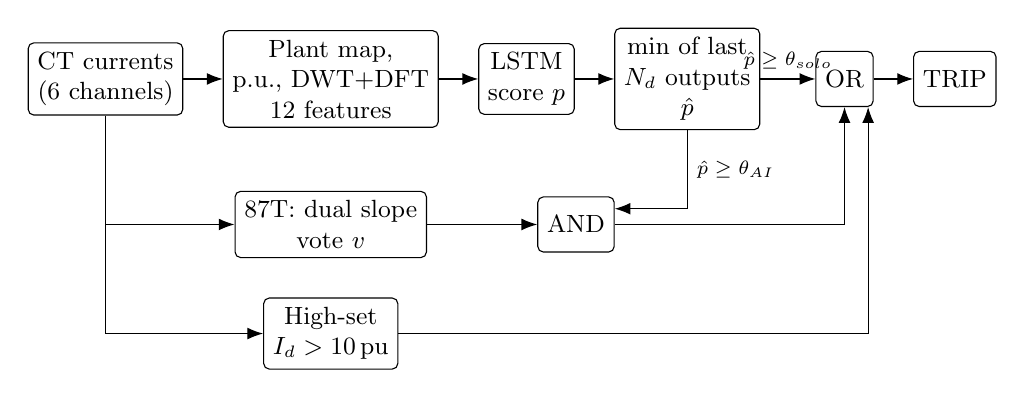
\begin{tikzpicture}[node distance=5mm, box/.style={draw,rounded corners=2pt,minimum height=7mm,align=center,font=\small}, arr/.style={-{Latex[length=2mm]}}]
\node[box] (ct) {CT currents\\(6 channels)};
\node[box,right=of ct] (dwt) {Plant map,\\p.u., DWT+DFT\\12 features};
\node[box,right=of dwt] (lstm) {LSTM\\score $p$};
\node[box,right=of lstm] (min) {min of last\\$N_d$ outputs\\$\hat p$};
\node[box,below=8mm of dwt] (87) {87T: dual slope\\vote $v$};
\node[box,below=of 87] (hs) {High-set\\$I_d>10$\,pu};
\node[box,right=14mm of 87] (and) {AND};
\node[box,right=of min,xshift=2mm] (or) {OR};
\node[box,right=of or] (trip) {TRIP};
\draw[arr] (ct)--(dwt); \draw[arr] (dwt)--(lstm); \draw[arr] (lstm)--(min);
\draw[arr] (ct.south) |- (87.west); \draw[arr] (ct.south) |- (hs.west);
\draw[arr] (87)--(and); \draw[arr] (min.south) |- ([yshift=2mm]and.east) node[pos=.25,right,font=\scriptsize] {$\hat p\geq\theta_{AI}$};
\draw[arr] (and.east)-|(or.south) ; \draw[arr] (min)--(or) node[midway,above,font=\scriptsize] {$\hat p\geq\theta_{solo}$};
\draw[arr] (hs.east)-|([xshift=3mm]or.south);
\draw[arr] (or)--(trip);
\end{tikzpicture}
\caption{Dual-path relay. $\hat p$ is the minimum of the last $N_d$ network outputs; the three inputs of the OR are the AI-gated 87T vote, the AI-alone path and the high-set element.}\label{fig:relay}
\end{figure}
The relay trips when
\begin{equation}
\text{TRIP}=\text{HighSet}\;\vee\;\big(v\wedge \hat p\ge\theta_{AI}\big)\;\vee\;\big(\hat p\ge\theta_{solo}\big),
\label{eq:trip}
\end{equation}
where $v$ is the any-phase vote of the dual-slope 87T (pickup 0.30\,pu, slopes 25\,\% and 60\,\%, breakpoint 3\,pu), and $\hat p$ is the minimum of the last $N_d=\dwellN$ network outputs (12.5\,ms at 1600\,Hz). The AI-alone path exists because a fault below the 87T pickup produces no vote; the high-set element ($I_d>10$\,pu) trips without the network. In the final plant-A model $\theta_{AI}=\thrAi$ and $\theta_{solo}=\thrSolo$.

\subsection{Thresholds}
Both thresholds are chosen by a plateau rule on the validation traces of each model: the lowest threshold in the longest range over which validation dependability and security stay within fixed tolerances of their maximum. No test or OOD trace is used.

\section{Evaluation protocol}
\label{sec:protocol}
\textbf{Splits.} Folds are stratified by scenario and contain whole traces (not windows); duplicate traces are removed by waveform fingerprint. Five folds are repeated with three seeds, giving \cvNfold{} fold-models; within each training set 15\,\% of the traces are held out for threshold tuning.
\textbf{Labels.} The fault label starts at the fault inception time of the generator (verified against the simulated waveform) plus eight samples; healthy traces are negative throughout. A trip before inception counts as a pre-fault trip and as a miss.
\textbf{Undetectable faults.} Faults whose rise of the compensated differential after inception is below 0.05\,pu are not part of the headline dependability; they are reported separately.
\textbf{OOD.} The final model (trained on all main-set traces except its validation share) scores the OOD set once.
\textbf{Baselines.} The unrestrained 87T, a harmonic-restrained 87T with per-phase 2nd/5th-harmonic restraint (15\,\% and 35\,\%), and five literature classifiers (SVM, ANN, random forest, 1D-CNN, GRU on the same wavelet features), trained on the same folds with the same dwell filter and high-set element.
\textbf{Statistics.} Paired McNemar tests \citep{mcnemar1947,dietterich1998} (continuity correction) on traces matched by identity, and Wilson 95\,\% intervals \citep{wilson1927}. Dependability is computed over fault traces and security over healthy traces.
\textbf{Closed loop.} Selected traces are replayed in the Simulink model with the network active; the decisions and trip times are compared with the Python mirror of the relay.

\section{Results}
\label{sec:results}
\subsection{Plant A: ablation}
\begin{table}[H]\centering
\caption{Ablation and architecture performance comparison on the publication dataset (grouped 5-fold CV, 3 random seeds, 15 fold-models total, $N_{\text{eval}}$ per repetition given in the note).}\label{tab:6.1_ablation}
\resizebox{\textwidth}{!}{%
\begin{tabular}{@{}lccccc@{}}\toprule
\textbf{Protection Architecture} & \textbf{Dependability (\%)} & \textbf{Security (\%)} & \textbf{Median $T_{op}$ (ms)} & \textbf{$\le$ 2 Cycles (\%)} & \textbf{Pre-Fault Trips}\\ \midrule
Conventional 87T Alone & 80.34 & 63.41 & 1.2 & 100.0 & 333.0\\
Standalone LSTM Alone & 97.68 & 95.60 & 15.6 & 96.3 & 4.0\\
Hybrid (87T-Gate Only) & 88.38 & 99.43 & 16.2 & 95.1 & 0.0\\
\textbf{Hybrid + AI-Alone Path (Proposed)} & \textbf{92.99 $\pm$ 3.60} & \textbf{98.96 $\pm$ 0.81} & \textbf{16.2} & \textbf{93.0} & \textbf{0.0}\\
\bottomrule
\end{tabular}%
}
\vspace{3pt}\raggedright\footnotesize\textit{Note:} Conventional 87T denotes unaugmented dual-slope percentage differential ($I_{pickup} = 0.30$\,pu, $S_1 = 25\%$, $S_2 = 60\%$, $I_{bp} = 3.0$\,pu) without startup delay. $N_{\text{eval}} = 3238$ traces per repetition; $\pm$: standard deviation over the 15 fold-models.
\end{table}
Pooled over \cvNfold{} fold-models, the relay with the AI-alone path reaches \cvHybDep\,\% dependability and \cvHybSec\,\% security (\cvHybMissed{} missed faults, \cvHybFalse{} false trips); the standard deviation over fold-models is \cvHybDepSD{} and \cvHybSecSD{} points. Without the AI-alone path the 87T-gated relay reaches \cvGateDep\,\% and \cvGateSec\,\%; the network alone reaches \cvLstmDep\,\% and \cvLstmSec\,\% with \cvLstmFalse{} false trips. The unrestrained 87T reaches \cvTaDep\,\% and \cvTaSec\,\%; its false trips are inrush and over-excitation, as expected without harmonic restraint.

\subsection{Baselines and statistics}
The per-phase harmonic-restrained 87T reaches \cvHarmDep\,\% dependability and \cvHarmSec\,\% security on the same traces. In the first repetition, which the paired test uses, the relay reaches \mcPDepProp\,\% dependability and \mcPSecProp\,\% security against \mcPDepBase\,\% and \mcPSecBase\,\% for the harmonic 87T. Against it the relay is better on dependability (\mcPDepWins{} traces correct only for the relay, \mcPDepLoss{} only for the harmonic 87T, $p=\mcPDepP$) and not different on security (\mcPSecWins{} against \mcPSecLoss{}, $p=\mcPSecP$). Against the unrestrained 87T both differences are significant (dependability $p=\mcUDepP$, security $p=\mcUSecP$).
\begin{table}[H]\centering
\caption{Paired McNemar statistical significance tests ($df=1$, with continuity correction) comparing the Proposed Hybrid Relay against conventional differential relay baselines.}\label{tab:6.3_stats}
\small
\begin{tabular}{@{}llccccc@{}}\toprule
\textbf{Baseline Model} & \textbf{Metric} & \textbf{Proposed} & \textbf{Baseline} & \textbf{Discordant ($b/c$)} & \textbf{McNemar $\chi^2$} & \textbf{$p$-Value}\\ \midrule
Conventional 87T Alone & Dependability & 93.92\% & 80.34\% & 179 / 9 & 151.92 & $< 10^{-10}$\\
Conventional 87T Alone & Security & 99.14\% & 63.41\% & 718 / 8 & 692.40 & $< 10^{-10}$\\
\midrule
Harmonic 87T (Per-Phase) & Dependability & 93.92\% & 85.93\% & 101 / 1 & 96.09 & $< 10^{-10}$\\
Harmonic 87T (Per-Phase) & Security & 99.14\% & 99.40\% & 12 / 17 & 0.55 & 4.5826e-01\\
\bottomrule
\end{tabular}
\vspace{3pt}\raggedright\footnotesize\textit{Note:} $b$: traces correctly classified by Proposed but failed by Baseline; $c$: traces correctly classified by Baseline but failed by Proposed. 3 of 4 comparisons are significant at $\alpha = 0.001$; not significant: proposed vs harmonic 87t per phase security (p = 0.458).
\end{table}
Table~\ref{tab:lit} places the five literature classifiers beside the relay. Used as direct-trip classifiers they reach 97--98\,\% dependability and 96--97\,\% security; placed in the dual-path relay, all of them reach 92--94\,\% dependability and 98--99\,\% security. The differences between the learned models inside the relay are small; the difference between the two operating modes is larger than the difference between models.
\begin{table}[t]\centering\small
\caption{Literature classifiers and the proposed network on the same folds (first repetition), as direct trip and inside the dual-path relay.}\label{tab:lit}
\resizebox{\textwidth}{!}{\begin{tabular}{@{}llrrrrr@{}}\toprule
Model & Mode & Parameters & Dep.\,(\%) & Sec.\,(\%) & Median $T_{op}$ (ms) & False trips\\ \midrule
Conventional 87T & direct trip & --- & 80.34 & 63.41 & 1.2 & 727\\
Wavelet-SVM & direct trip & 5{,}880 & 84.01 & 74.23 & 15.6 & 512\\
Wavelet-SVM & in the dual-path relay & 5{,}880 & 80.82 & 98.24 & 18.1 & 35\\
Wavelet-ANN & direct trip & 5{,}441 & 97.12 & 96.28 & 16.2 & 74\\
Wavelet-ANN & in the dual-path relay & 5{,}441 & 92.57 & 99.09 & 16.9 & 18\\
Wavelet-RF & direct trip & 37{,}802 & 96.32 & 96.88 & 16.2 & 62\\
Wavelet-RF & in the dual-path relay & 37{,}802 & 92.09 & 99.25 & 19.4 & 15\\
1D-CNN & direct trip & 14{,}561 & 97.52 & 96.73 & 16.2 & 65\\
1D-CNN & in the dual-path relay & 14{,}561 & 92.25 & 99.14 & 18.1 & 17\\
Wavelet-GRU & direct trip & 44{,}354 & 98.40 & 96.53 & 15.0 & 69\\
Wavelet-GRU & in the dual-path relay & 44{,}354 & 93.29 & 99.04 & 15.6 & 19\\
Standalone LSTM & direct trip & 58{,}241 & 97.92 & 96.78 & 15.6 & 64\\
Proposed Hybrid DWT-LSTM & in the dual-path relay & 58{,}241 & 93.92 & 99.14 & 16.2 & 17\\
\bottomrule
\end{tabular}}
\end{table}

\subsection{Categories}
\begin{table}[H]\centering
\caption{Performance breakdown across all 16 scenario categories under grouped 5-fold CV (Proposed Hybrid + AI-Alone Path vs Baselines).}\label{tab:6.2_categories}
\setlength{\tabcolsep}{4.5pt}\small
\resizebox{\textwidth}{!}{%
\begin{tabular}{@{}lcccccc@{}}\toprule
\textbf{Scenario Category} & \textbf{Traces ($N$)} & \textbf{Expected} & \textbf{Proposed [95\% Wilson CI]} & \textbf{LSTM Alone} & \textbf{87T Alone} & \textbf{Med.\,$T_{op}$}\\ \midrule
Evolving & 80 & Trip & 100.0 [98.4, 100.0] & 100.0 & 100.0 & 16.2\,ms\\
External CT-sat & 302 & Block & 98.7 [97.7, 99.2] & 93.6 & 66.9 & ---\\
External HiZ & 60 & Block & 100.0 [97.9, 100.0] & 100.0 & 100.0 & ---\\
External in inrush & 100 & Block & 88.3 [84.2, 91.5] & 78.7 & 0.0 & ---\\
External solid & 440 & Block & 98.9 [98.2, 99.4] & 90.2 & 100.0 & ---\\
Fault in inrush & 111 & Trip & 100.0 [98.9, 100.0] & 98.8 & 0.0 & 28.1\,ms\\
Inrush loaded & 192 & Block & 100.0 [99.3, 100.0] & 99.7 & 0.0 & ---\\
Inrush no-load & 200 & Block & 99.8 [99.1, 100.0] & 98.8 & 0.0 & ---\\
Internal CT-sat & 121 & Trip & 100.0 [99.0, 100.0] & 100.0 & 100.0 & 16.2\,ms\\
Internal HV-side & 198 & Trip & 100.0 [99.4, 100.0] & 100.0 & 100.0 & 3.8\,ms\\
Internal HiZ & 155 & Trip & 65.8 [61.4, 70.0] & 87.1 & 51.0 & 25.6\,ms\\
Internal LV solid & 506 & Trip & 94.7 [93.5, 95.7] & 99.8 & 88.3 & 16.9\,ms\\
Normal & 303 & Block & 100.0 [99.6, 100.0] & 100.0 & 100.0 & ---\\
Over-excitation & 310 & Block & 100.0 [99.6, 100.0] & 100.0 & 63.2 & ---\\
Recovery inrush & 80 & Block & 100.0 [98.4, 100.0] & 99.2 & 73.8 & ---\\
SOTF & 80 & Trip & 90.0 [85.6, 93.2] & 91.7 & 100.0 & 21.2\,ms\\
\bottomrule
\end{tabular}%
}
\vspace{3pt}\raggedright\footnotesize\textit{Note:} Wilson 95\% confidence intervals computed over unique evaluated traces. Total unique traces = 3238.
\end{table}
The weakest categories of the relay are internal high-impedance faults (\catHiz\,\% correct), external faults during inrush (\catExtInrush\,\%) and switch-on-to-fault (\catSotf\,\%); internal solid faults on the LV side are \catLvSolid\,\%.

\subsection{Out-of-distribution}
\begin{table}[H]\centering
\caption{Single-pass out-of-distribution (OOD) stress evaluation on 299 held-out traces with zero retraining or threshold adaptation.}\label{tab:6.4_ood}
\small
\begin{tabular}{@{}llcccc@{}}\toprule
\textbf{Stress Condition Block} & \textbf{Operating Range} & \textbf{Faults ($N$)} & \textbf{Dep.\,(\%)} & \textbf{Healthy ($N$)} & \textbf{Sec.\,(\%)}\\ \midrule
Block 1: Extreme Loading & 1--10\% and 110--130\% rated load & 30 & 100.0 & 30 & 96.7\\
Block 2: Weak Source + Frequency Drift & Source $Z \times 3$, $f = 49.5 / 50.5$\,Hz & 30 & 100.0 & 30 & 100.0\\
Block 3: Extreme CT Burden Saturation & CT burden 8--12$\times$ nominal & 30 & 100.0 & 30 & 96.7\\
Block 4: Severe Overexcitation + Flux & $V = 1.5$--$1.6$\,pu, $\psi_{\text{rem}} = 0.90$\,pu & 30 & 96.7 & 30 & 93.3\\
Block 5: Severe Noise + CT Mismatch & BLWN noise 5\%, CT mismatch $\pm 8\%$ & 29 & 93.1 & 30 & 93.3\\
\midrule
\textbf{Overall OOD Performance} & \textbf{All 5 Stress Blocks Combined} & \textbf{149} & \textbf{98.0} & \textbf{150} & \textbf{96.0}\\
\bottomrule
\end{tabular}
\vspace{3pt}\raggedright\footnotesize\textit{Note:} Median operating time across all OOD internal faults: 17.5\,ms. Pre-fault trips: 0.
\end{table}
On the \oodN{} OOD traces (scored once) the relay reaches \oodDep\,\% dependability and \oodSec\,\% security (\oodMissed{} missed faults, \oodFalse{} false trips); the weakest block for security is over-excitation (\oodBlockDSec\,\%).

\subsection{Plant B}
\begin{table}[H]\centering
\caption{Cross-plant generalization and transfer capability on Plant B (40\,MVA, 132/33\,kV, Dyn11, 1\,A CTs).}\label{tab:6.8_plant_b}
\small
\begin{tabular}{@{}llcccc@{}}\toprule
\textbf{Experiment Type} & \textbf{Protection Model} & \textbf{Dependability (\%)} & \textbf{Security (\%)} & \textbf{Median $T_{op}$} & \textbf{False Trips}\\ \midrule
\multicolumn{6}{@{}l}{\textit{Panel A: Zero-Shot Transfer on Plant B (Model Trained on Plant A Alone)}} \\ \midrule
Zero-Shot & Conventional 87T Alone & 89.45 & 62.04 & 3.8\,ms & 290\\
Zero-Shot & Harmonic Restrained 87T & 94.12 & 98.95 & 14.1\,ms & 8\\
Zero-Shot & \textbf{Proposed DWT-LSTM (Zero-Shot)} & 92.70 & 88.35 & 14.4\,ms & 89\\
\midrule
\multicolumn{6}{@{}l}{\textit{Panel B: Cross-Plant Training (Pooled Plant A + Plant B, 5-Fold CV)}} \\ \midrule
Cross-Plant & Pooled Plants A + B & 94.78 & 98.22 & 15.0\,ms & ---\\
Cross-Plant & Plant A Evaluation & 94.56 & 98.79 & 15.6\,ms & ---\\
Cross-Plant & Plant B Evaluation & 95.33 & 96.73 & 13.8\,ms & ---\\
\midrule
\multicolumn{6}{@{}l}{\textit{Panel C: Leave-One-Plant-Out Transfer}} \\ \midrule
Leave-One-Out & Train Plant A $\rightarrow$ Test Plant B & 93.10 & 89.79 & 13.8\,ms & 78\\
Leave-One-Out & Train Plant B $\rightarrow$ Test Plant A & 62.51 & 97.28 & 15.6\,ms & 54\\
\bottomrule
\end{tabular}
\vspace{3pt}\raggedright\footnotesize\textit{Note:} Plant B features computed using Dyn11 per-unit differential transformation. Unchanged detection thresholds ($	heta_{	ext{ai}} = 0.9950$, $	heta_{	ext{solo}} = 0.9980$, dwell $= 20$).
\end{table}
The model trained on plant~A, applied to plant~B without retraining and with its thresholds frozen, reaches \zsPropDep\,\% dependability and \zsPropSec\,\% security (\zsPropFalse{} false trips among \zsNhealthy{} healthy traces); the harmonic 87T reaches \zsHarmDep\,\% and \zsHarmSec\,\% (\zsHarmFalse{} false trips). A trip-path analysis shows that \tpFalseSolo{} of the \tpFalseAll{} false trips come first through the AI-alone path, mostly on external faults with CT saturation (\tpFalseExt{} traces); without that path the zero-shot relay reaches \tpNoSoloDep\,\% and \tpNoSoloSec\,\%. Training on both plants gives \cpDep\,\% and \cpSec\,\% (plant~A subset \cpADep\,\%/\cpASec\,\%, plant~B subset \cpBDep\,\%/\cpBSec\,\%). Trained on plant~A and tested on plant~B: \looABDep\,\%/\looABSec\,\%; trained on plant~B and tested on plant~A: \looBADep\,\%/\looBASec\,\%.

\subsection{Closed loop and execution time}
\begin{table}[H]\centering
\caption{Simulink dynamic closed-loop simulation vs.\ offline Python relay mirror across 50 dynamic traces (held-out validation + OOD).}\label{tab:6.5_closed_loop}
\small
\begin{tabular}{@{}lcccc@{}}\toprule
\textbf{Test Evaluation Set} & \textbf{Traces ($N$)} & \textbf{Decision Agreement} & \textbf{Median $|\Delta t|$} & \textbf{Max $|\Delta t|$}\\ \midrule
Held-Out Validation Traces & 25 & 25 / 25 (100.0\%) & 0.00\,ms & 0.30\,ms\\
Out-of-Distribution (OOD) Traces & 25 & 25 / 25 (100.0\%) & 0.00\,ms & 0.12\,ms\\ \midrule
\textbf{Combined Total Suite} & \textbf{50} & \textbf{50 / 50 (100.0\%)} & \textbf{0.00\,ms} & \textbf{0.30\,ms}\\
\bottomrule
\end{tabular}
\vspace{3pt}\raggedright\footnotesize\textit{Note:} Ground-truth trip accuracy: Simulink 49 / 50, Python mirror 49 / 50. |$\Delta t$| over the 24 traces tripped by both.
\end{table}
In the Simulink closed loop, \clAgree{} of \clTotal{} decisions agree with the Python mirror; the median absolute trip-time difference is \clDtMed\,ms (maximum \clDtMax\,ms). Against the ground truth Simulink is correct on \clSimOk{} of \clTotal{} traces; \clNfail{} traces fail the combined decision-and-30\,ms check. The 12-case suite on plant~B passes \clBPass{} of \clBTotal{}.
\begin{table}[H]\centering
\caption{Measured real-time execution latency benchmark over 10{,}000 timed streaming evaluations on AMD Ryzen 7 7700 (single thread).}\label{tab:6.6_latency}
\small
\begin{tabular}{@{}lcccccc@{}}\toprule
\textbf{Implementation / Relay Stage} & \textbf{Mean ($\mu$s)} & \textbf{Std ($\mu$s)} & \textbf{Median ($\mu$s)} & \textbf{95th-Pctl ($\mu$s)} & \textbf{99th-Pctl ($\mu$s)} & \textbf{Max ($\mu$s)}\\ \midrule
\multicolumn{7}{@{}l}{\textit{Panel A: Python 3.11 with ONNX Runtime 1.27}} \\ \midrule
Feature Extraction (PyWavelets + NumPy) & 22.3 & 4.5 & 21.7 & 23.0 & 38.5 & 265.3\\
LSTM Inference (ONNX Runtime) & 91.1 & 10.9 & 88.8 & 101.0 & 135.9 & 319.4\\
\textbf{Combined ONNX Pipeline} & \textbf{143.1} & \textbf{15.4} & \textbf{139.6} & \textbf{150.3} & \textbf{218.9} & \textbf{438.1}\\
\midrule
\multicolumn{7}{@{}l}{\textit{Panel B: Standalone Compiled ANSI C (MinGW-w64 GCC 16.1, -O3 -mavx2 -mfma)}} \\ \midrule
Feature Extraction (Matrix DWT + FFT) & 1.1 & 0.1 & 1.0 & 1.3 & 1.5 & 11.0\\
LSTM Inference (2-Layer + Attention) & 178.3 & 12.4 & 176.0 & 187.1 & 232.2 & 543.2\\
\textbf{Combined Standalone C Pipeline} & \textbf{178.3} & \textbf{12.5} & \textbf{175.9} & \textbf{185.7} & \textbf{228.9} & \textbf{376.9}\\
\bottomrule
\end{tabular}
\vspace{3pt}\raggedright\footnotesize\textit{Note:} Real-time sampling period at 1{,}600\,Hz: 625.0\,$\mu$s. Median execution times occupy 22.3\% (ONNX) and 28.1\% (ANSI C) of the sample budget. The C source is hand-written (emitted by a Python script), not MATLAB Coder or Embedded Coder output, and was timed on the development PC, not on a relay processor.
\end{table}
The feature extraction and network take a median of \latOnnxMed\,$\mu$s with ONNX Runtime and \latCMed\,$\mu$s in hand-written ANSI C (99th percentile \latCPnn\,$\mu$s) on a development PC, against a sample period of \latPeriod\,$\mu$s. These figures are not measurements on a relay processor.

\subsection{A design variant tested afterwards}
Using the per-phase harmonic-restrained 87T as the gate of the relay (decided after the results above; protocol fixed before the run) gives \eOneDep\,\% dependability and \eOneSec\,\% security in cross-validation (dependability: \eOneDepWins{} against \eOneDepLoss{} discordant traces, $p=\eOneDepP$), \eOneOodSec\,\% security on the OOD set, and no change in the zero-shot false trips. The variant is not adopted.

\section{Limitations}
\label{sec:limits}
The study is a simulation of two transformers with terminal faults; there is no hardware-in-the-loop test, no field data, no inter-turn faults and no CT remanence. Internal high-impedance faults are detected in \catHiz\,\% of traces. The model does not transfer to a different transformer without retraining. The relay's dependability is lower than that of the standalone networks and higher than that of the harmonic-restrained 87T; its security is equal to the latter's within the statistical resolution. Two plant~B physics criteria are not met (Section~\ref{sec:data}). The execution times are those of a development PC. Block-decomposition and Clarke-wavelet detectors \tc{} were not implemented and are not compared.

\section{Conclusion}
On a plant whose CTs are linear at nominal burden, a wavelet-feature LSTM used as a dual-path supervisor of the 87T matches the security of a per-phase harmonic-restrained 87T and raises dependability from \cvHarmDep\,\% to \cvHybDep\,\% on the same cross-validation traces, mainly on faults below the 87T pickup. It needs training on the protected plant or on a pool of plants. The evaluation protocol, the plant checks and the generators are in the repository.

\section*{Data and code availability}
Generators, models, evaluation code and logs: \url{https://github.com/SS-Abeer13/Hybrid-DWT-LSTM-Transformer-Relay}. Datasets and trained models are not stored in the repository because of their size and are regenerated by the scripts listed in its README.

\section*{Declarations}
Funding, competing interests, CRediT author statement and use of AI tools: to be completed by the authors.

\bibliographystyle{elsarticle-harv}
\bibliography{refs}
\end{document}
